\chapter{Wavelet-based Diffusion Model}

\section{Motivation}

The diffusion model presented in Chapter~3 operates directly on the density
fields in physical space. While this setting already provides a meaningful
baseline, it does not explicitly exploit the multi-scale structure discussed in
Chapter~2. Rayleigh--Taylor instability fields contain both large coherent
structures and fine localized fluctuations, and these components are not
equally easy to learn in pixel space. In particular, the small-scale features
associated with interface corrugations, local mixing events, and turbulent
details can be difficult to preserve when the model must simultaneously learn
the global morphology of the flow.

This observation motivates a second generative pipeline based on wavelet
coefficients. The main idea is to decompose each density field into an
approximation component, which captures the large-scale structure, and detail
components, which encode the local variations at a given resolution level. A
diffusion model is then trained not on the raw image itself, but on this
multi-resolution representation. The resulting surrogate is expected to better
capture the hierarchical organization of RTI fields and to produce samples that
preserve the dominant scales of the flow while remaining flexible enough to
reconstruct realistic fine-scale structures.

Compared with the baseline diffusion model, this approach introduces an
additional inductive bias: instead of learning the full spatial field at once,
the network learns to generate the wavelet detail coefficients conditioned on
the coarse approximation. 

An important difference also appears at the level of the prior. In the direct
diffusion model, generation starts from pure Gaussian noise having the same
spatial size as the target image. In the wavelet setting, the initial noise is
defined in coefficient space and is therefore smaller by a factor related to
the decomposition level $j$. In practice, a wavelet decomposition reduces the
resolution of the latent variable by approximately $2^j$ in each spatial
direction, so the generative model begins from a more compact prior while
still preserving the hierarchical structure needed to reconstruct the full
field.

\begin{figure}[H]
    \centering
    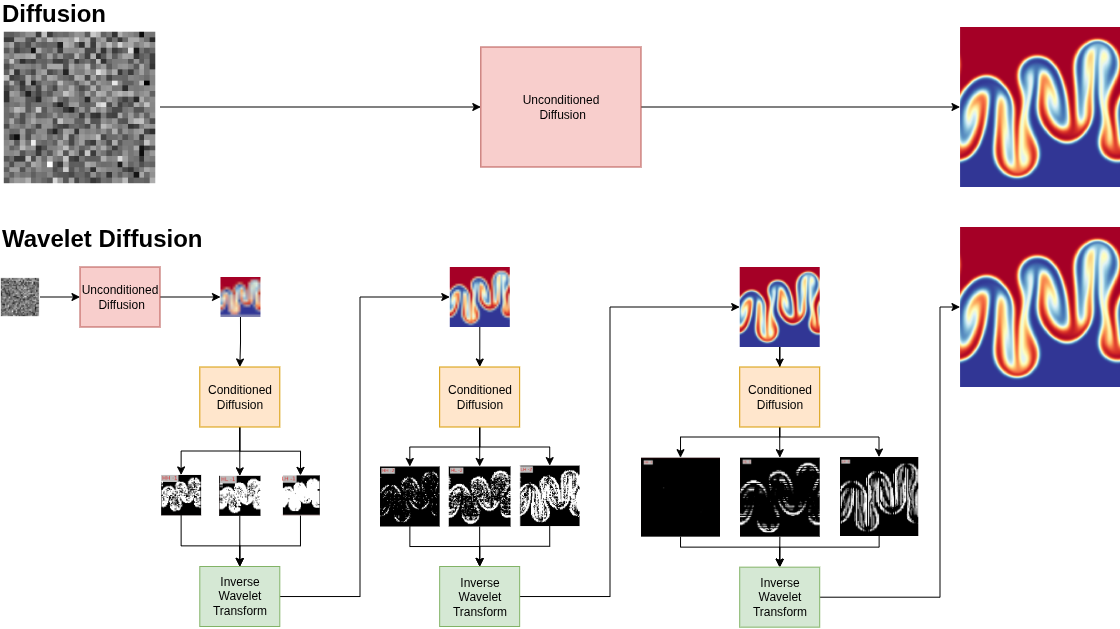
\includegraphics[width=0.95\textwidth]{figures/ch5/WaveletDiffusion.png}
    \caption{Comparison between direct diffusion and wavelet-based diffusion. In the wavelet case, the prior is defined on a lower-resolution latent representation before the inverse wavelet transform reconstructs the full field.}
    \label{fig:ch5_wavelet_diffusion_scheme}
\end{figure}





\section{Wavelet-based generative framework}

\subsection{Wavelet representation of RTI fields}

The wavelet pipeline begins with the preprocessing of the RTI dataset. The raw
density fields are first loaded from the simulation files and preprocessed
using the existing data augmentation routines. A two-dimensional discrete
wavelet transform is then applied to each image using a Daubechies-1 basis.

For a decomposition level $j$, each field is mapped to four coefficient maps:
the approximation coefficients $c_A$ and the horizontal, vertical, and
diagonal detail coefficients $c_H$, $c_V$, and $c_D$. In the implementation,
these four arrays are stacked into a tensor of shape $(N,4,H',W')$, where $N$
is the number of samples and $(H',W')$ is the spatial size of the wavelet
coefficients at the chosen level. The dataset is then split into training,
validation, and test subsets, and each split is saved independently as a PyTorch
tensor.

This representation preserves the most relevant multi-scale information while
reducing the learning problem to a structured tensor prediction task. In
practice, the decomposition also makes the notion of coarse-to-fine generation
explicit: the approximation channel plays the role of a low-frequency prior,
while the three detail channels contain the higher-frequency content that must
be synthesized.

\subsection{Conditional diffusion on wavelet coefficients}

The training data are loaded from the precomputed tensors and normalized
channel by channel using the statistics of the training split. This
normalization is important because the four wavelet channels do not share the
same numerical scale and would otherwise contribute unevenly to the
optimization process.

The model uses a conditional DDPM structure. The input to the U-Net is composed
of the approximation channel concatenated with the noisy detail channels. The
network predicts the noise applied to the detail coefficients, which means that
generation is guided by the coarse-scale information rather than being
unconditional. In other words, the model learns how to reconstruct the missing
fine-scale structure given the large-scale wavelet content.

The corresponding architecture is deliberately compact. The U-Net receives
four input channels in total, with one channel reserved for the prior
information and three channels corresponding to the target detail maps. The
network depth and the number of blocks per level remain modest so that training
is compatible with the size of the available RTI dataset. The diffusion
schedule itself follows the same principle as the baseline model, with a
discretized Markov process controlled by a linear noise schedule between
\texttt{min\_beta} and \texttt{max\_beta}.

During training, the loss is again the standard mean squared error between the
true noise and the noise predicted by the network. The model therefore learns a
denoising function conditioned on the coarse wavelet coefficients. Once
training is complete, the checkpoint and the preprocessing statistics are
stored in a configuration file so that sampling can be reproduced later without
ambiguity.

% \subsection{Generation procedure}

% The generation stage loads the trained checkpoint and the associated
% normalization parameters. A batch of wavelet coefficients is sampled from the
% validation set and the approximation channel is extracted as a condition.
% Starting from the conditional prior, the DDPM iteratively denoises the target
% detail channels and produces a synthetic coefficient tensor.

% The generated coefficients are then denormalized and saved to disk. This file
% can subsequently be converted back to image space by inverting the wavelet
% transform, which makes it possible to compare the generated fields with the
% reference RTI simulations both visually and quantitatively.

% Because the generation is conditioned on the low-frequency part of an existing
% sample, the model is not asked to invent the global structure from scratch. It
% instead focuses on reconstructing plausible local details compatible with the
% coarse-scale organization of the flow. This is a natural strategy for RTI
% fields, where the large-scale morphology strongly constrains the admissible
% small-scale fluctuations.

\begin{figure}[h]
    \centering
    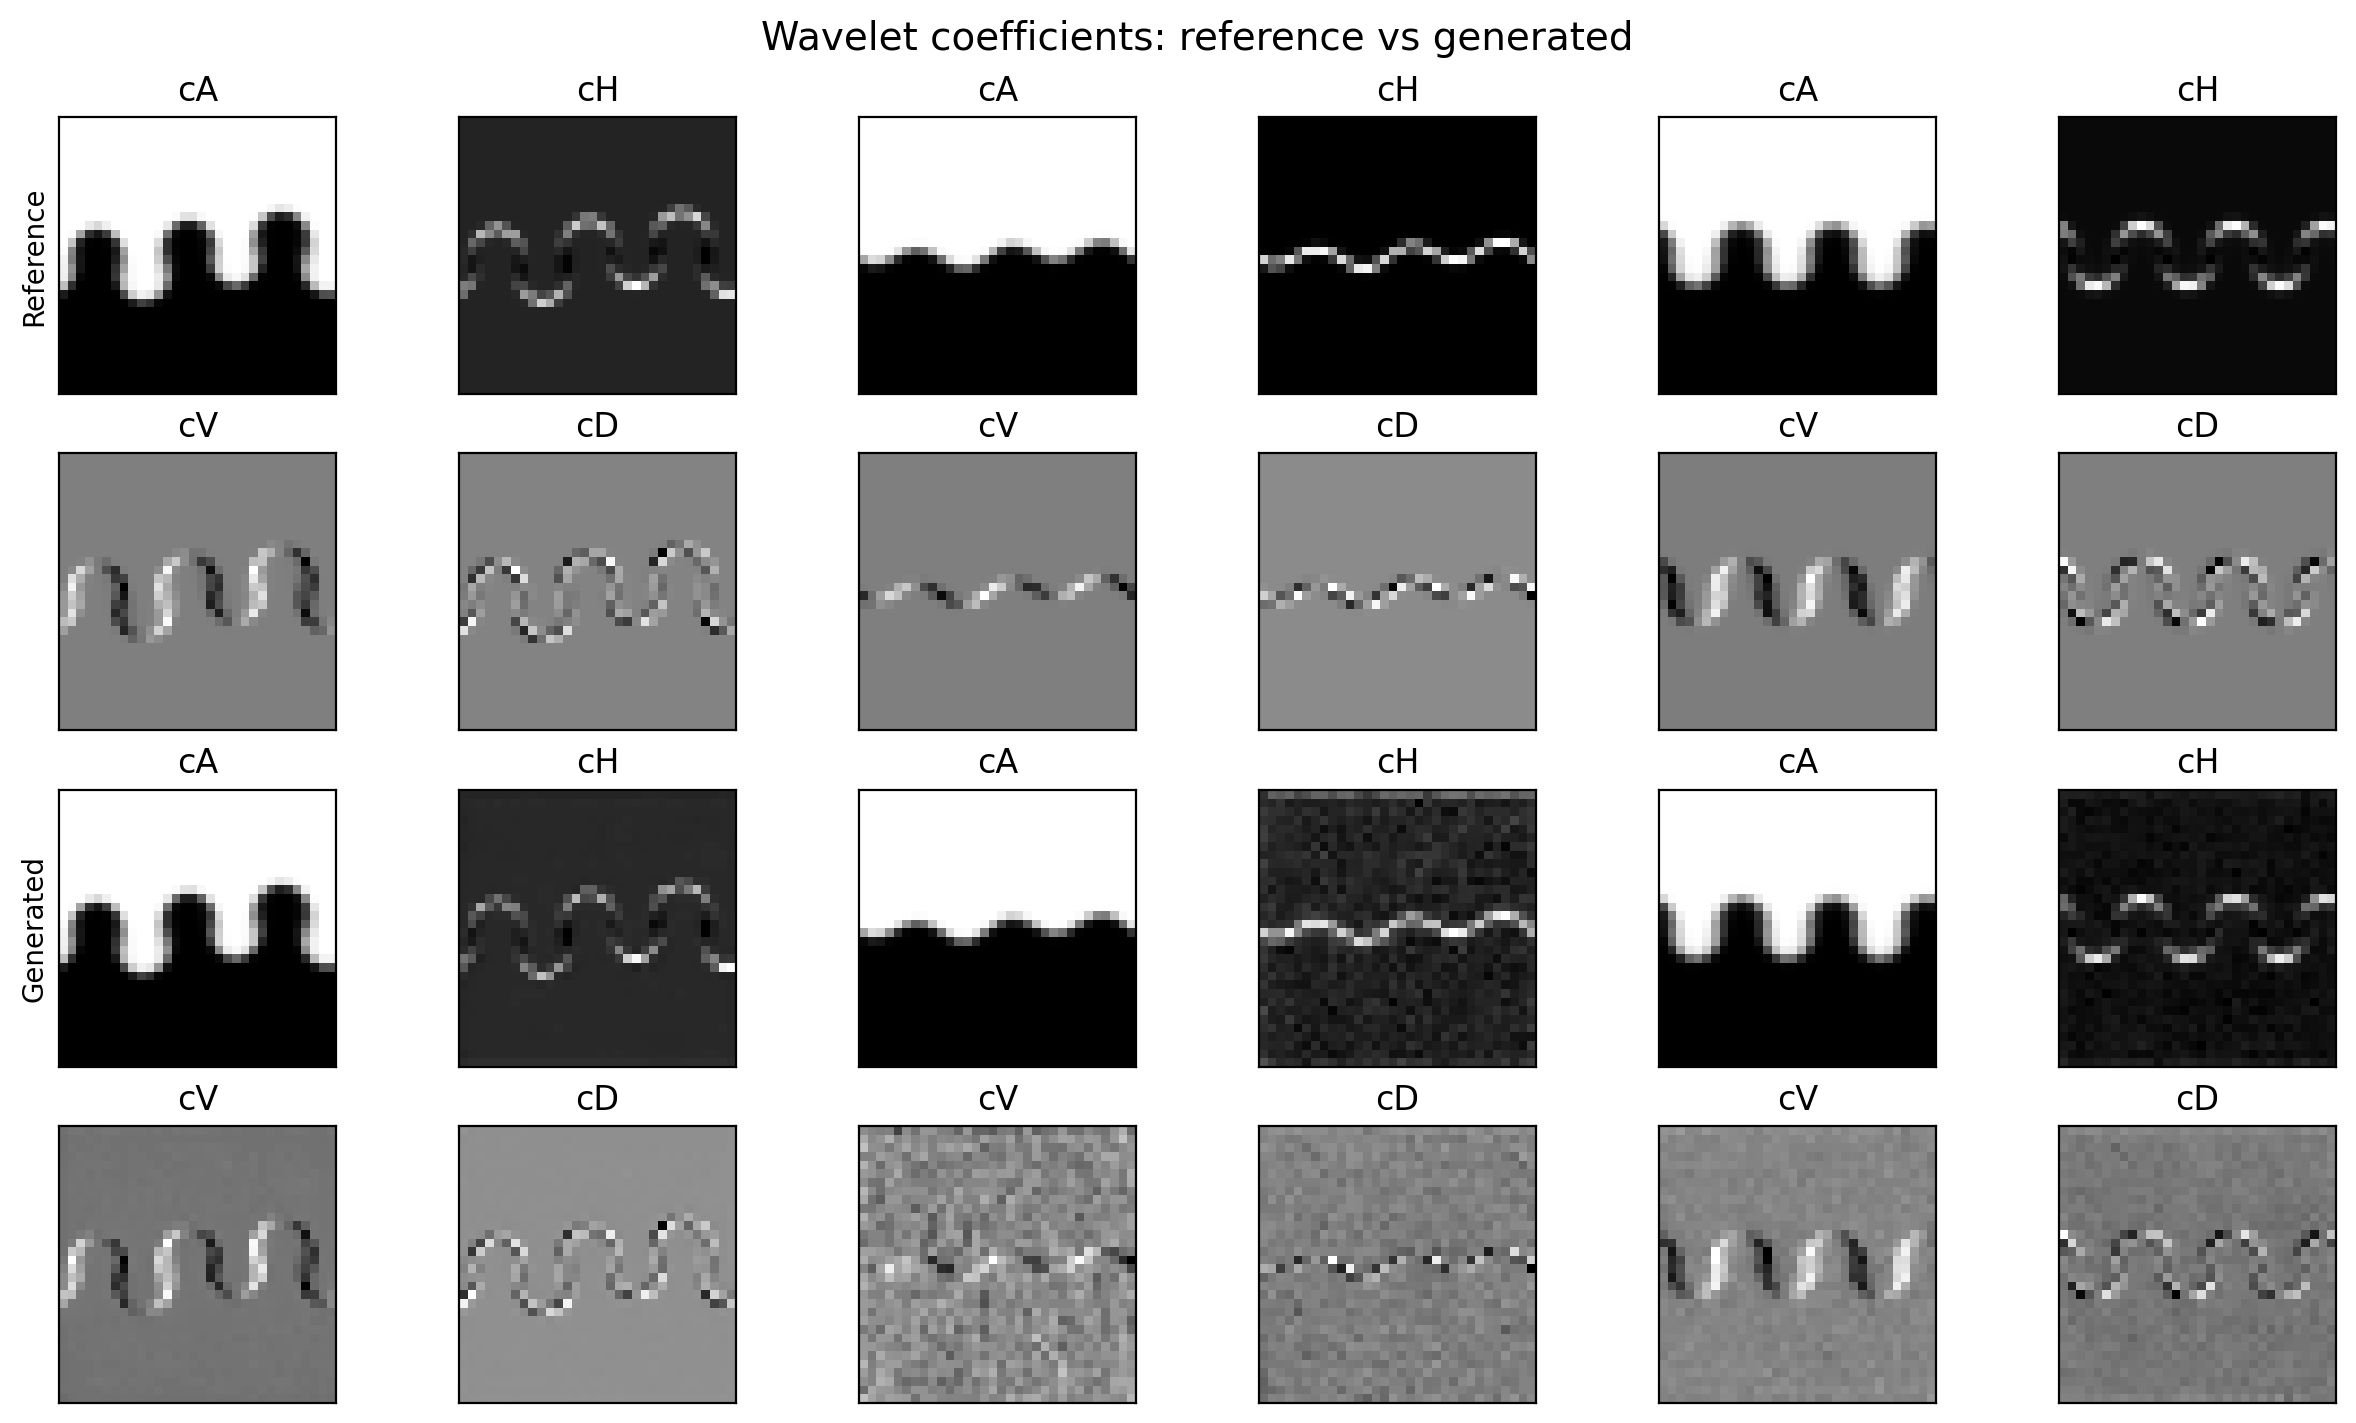
\includegraphics[width=0.95\textwidth]{figures/ch5/wavelet_coefficients_comparison.png}
    \caption{Comparison of wavelet coefficient maps between a reference RTI sample and a generated sample. The approximation channel and the three detail channels are shown separately.}
    \label{fig:ch5_wavelet_coefficients}
\end{figure}

\begin{figure}[h]
    \centering
    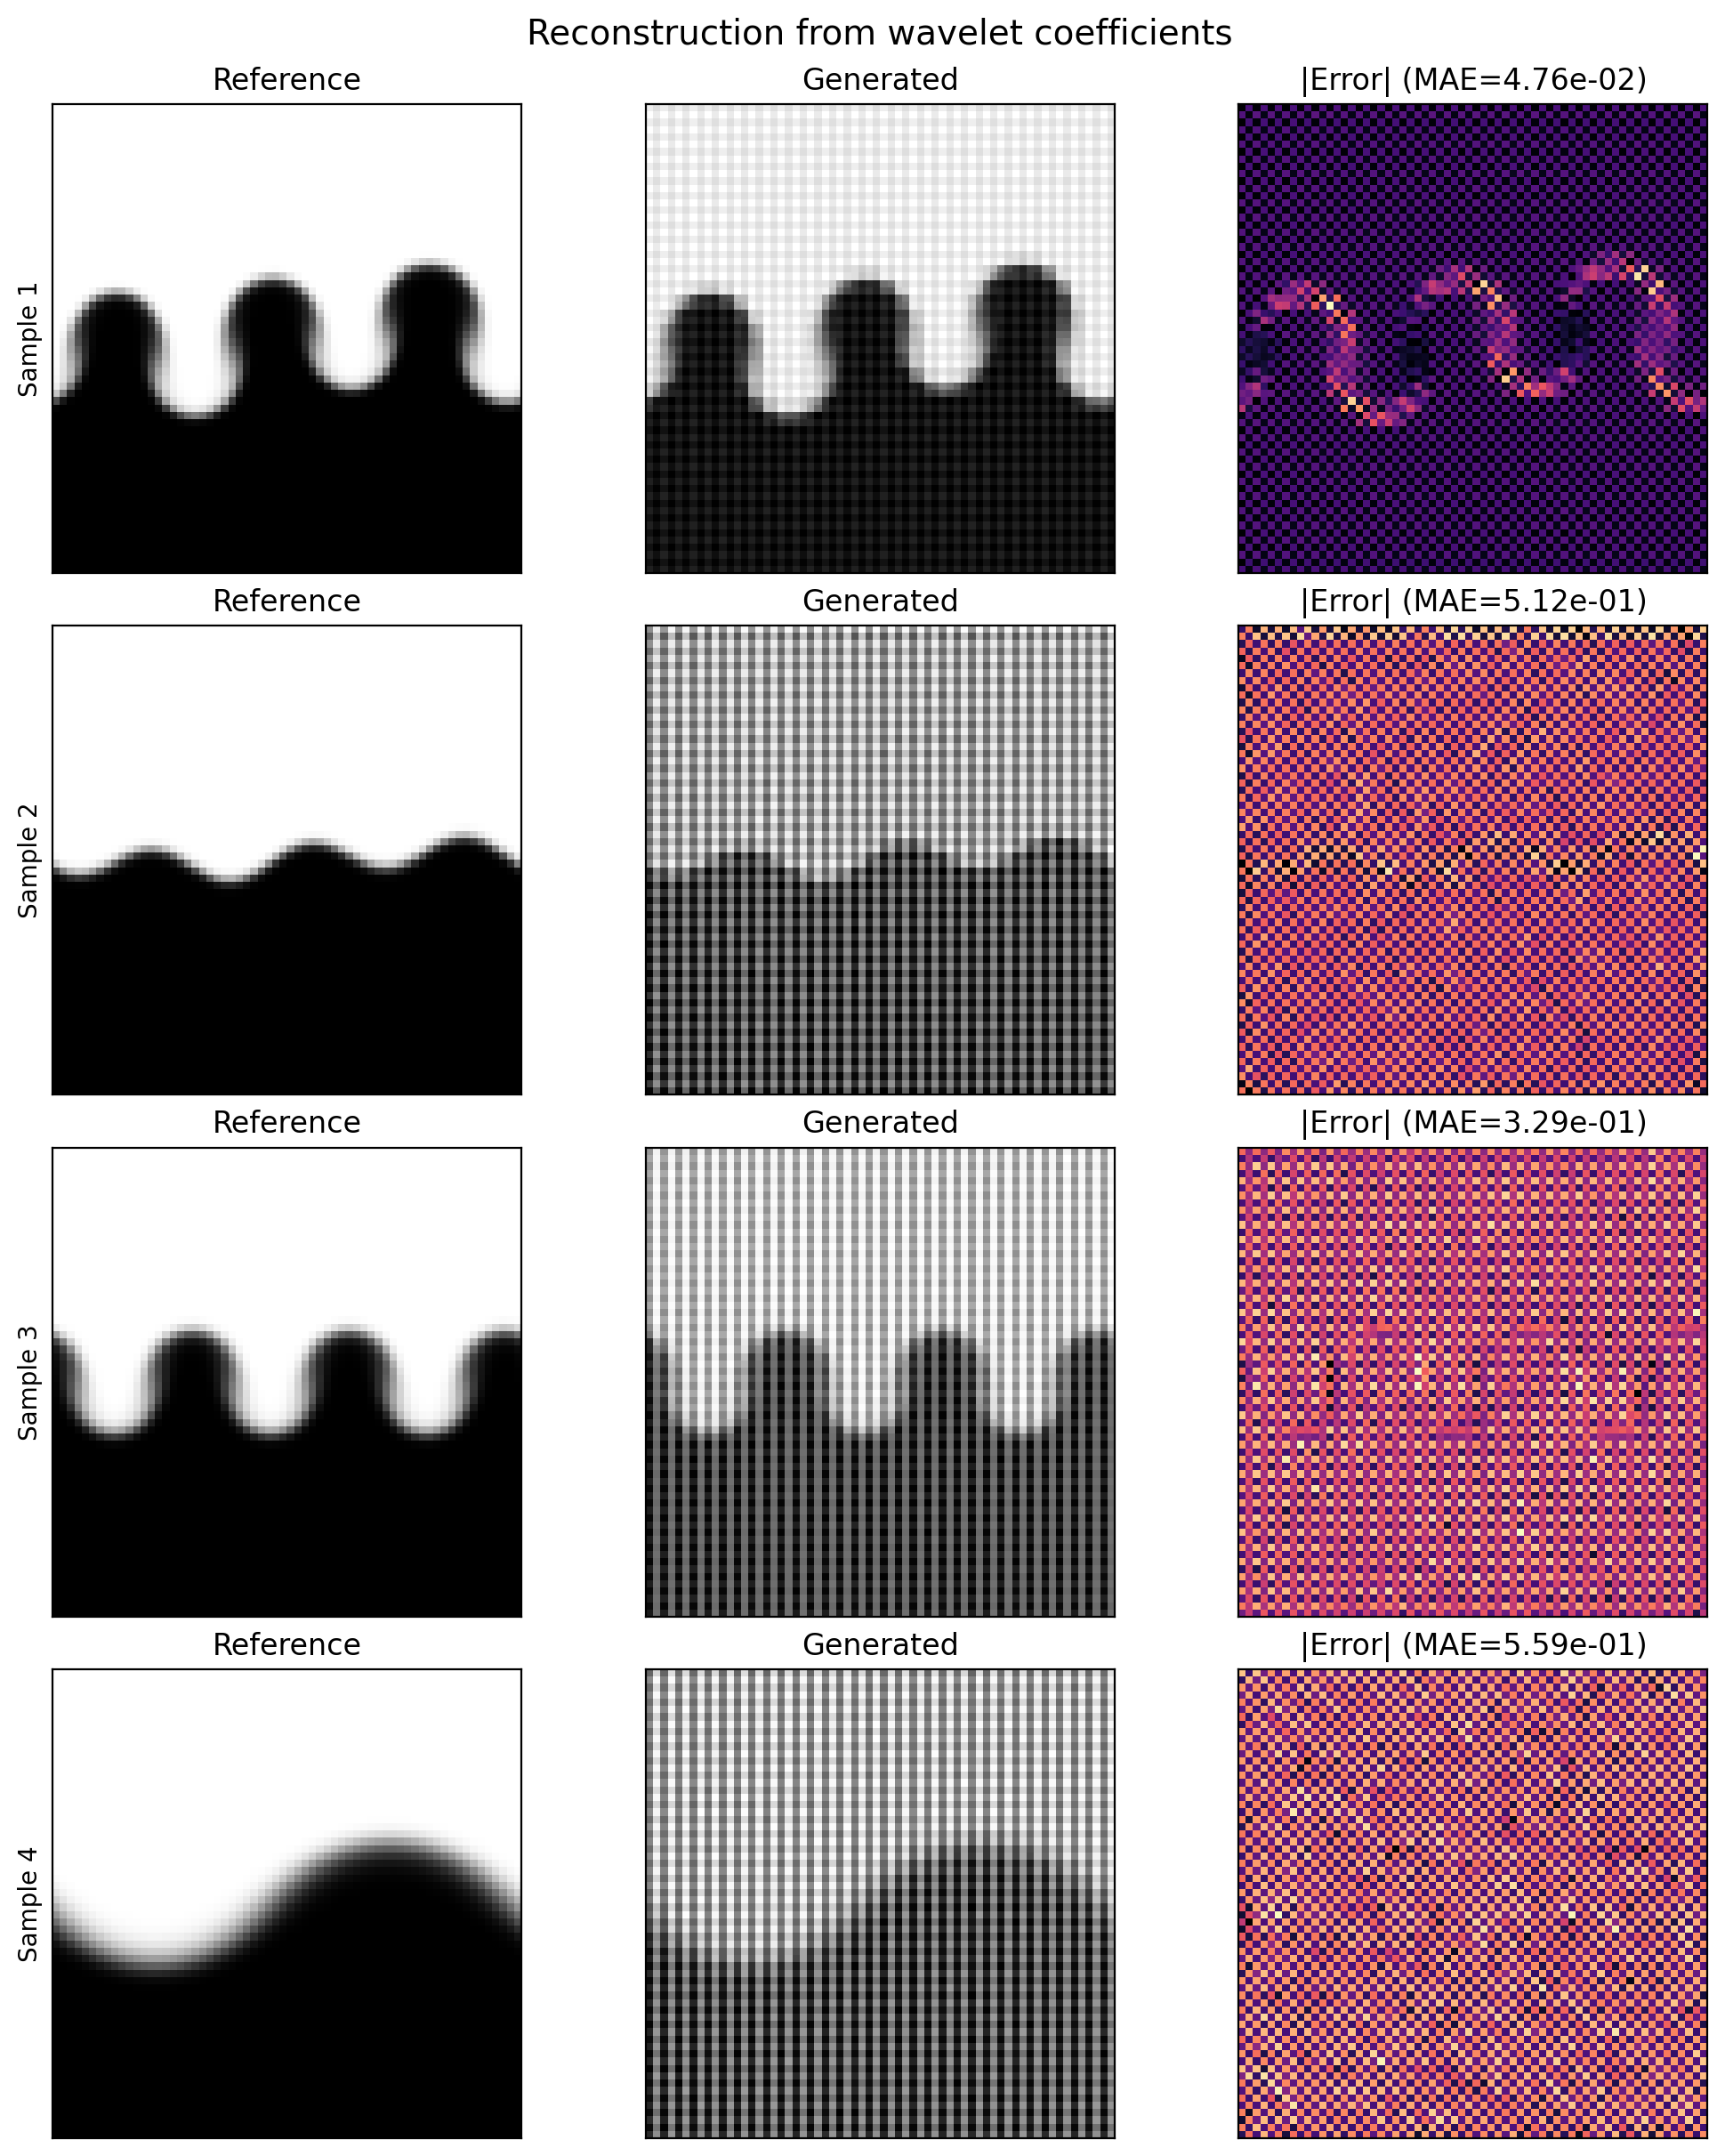
\includegraphics[width=0.65\textwidth]{figures/ch5/wavelet_reconstruction_comparison.png}
    \caption{Reconstruction of RTI fields from wavelet coefficients. For each example, the reference field, the generated field, and the absolute reconstruction error are shown.}
    \label{fig:ch5_wavelet_reconstruction}
\end{figure}

\section{Results and comparison with baseline diffusion}

At this stage, the evaluation of the wavelet-based diffusion model remains
primarily qualitative. The generated coefficient fields demonstrate that the
conditional diffusion framework is capable of learning non-trivial relationships
between the coarse approximation and the associated detail coefficients.
Furthermore, the wavelet representation provides an explicit separation of
spatial scales, making it possible to analyze the origin of reconstruction
errors and generated artifacts more precisely than in the direct image-space
formulation.

The reconstructed density fields nevertheless reveal several limitations of the
current implementation. While the large-scale organization imposed by the
approximation coefficients is generally preserved, the synthesized detail
coefficients often introduce artifacts and yield reconstructions that remain
visibly rougher than the reference DNS fields. In comparison, the baseline
diffusion model presented in Chapter~3 currently produces smoother samples that
are visually closer to the target distribution.

However, the present comparison remains incomplete. Although the visual quality
of the reconstructed fields clearly indicates that the current wavelet model
underperforms the baseline diffusion model, a quantitative assessment is still
required to characterize these differences rigorously. The phyFID score and the
line-based physical metrics introduced in Chapter~4 have not yet been computed
for the wavelet formulation. These indicators will provide a more objective
evaluation of the degradation observed in the generated samples and help
identify which physical and statistical properties are most affected by the
wavelet representation.

Despite its current limitations, the proposed formulation remains a promising
research direction. By explicitly separating coarse and fine scales, the model
introduces a physically meaningful inductive bias that is particularly well
suited to the multi-scale nature of Rayleigh--Taylor instability. Future work
will focus on refining the conditioning strategy, investigating alternative
wavelet decompositions and decomposition levels, and performing a complete
quantitative comparison with the baseline diffusion model. These developments
will determine whether wavelet-based diffusion can provide a competitive and
physically interpretable alternative to direct image-space generation.
